\documentclass[11pt,letterpaper]{article}
\usepackage[T1]{fontenc}
\usepackage[utf8]{inputenc}
\usepackage{mathptmx}
\usepackage[margin=1in]{geometry}
\usepackage{amsmath,amssymb}
\usepackage{enumitem}
\usepackage{graphicx}
\usepackage[table]{xcolor}
\usepackage{booktabs,longtable,array}
\usepackage[font=small,labelfont=bf,labelsep=period,justification=raggedright,singlelinecheck=false]{caption}
\usepackage{fancyhdr}
\usepackage{titlesec}
\usepackage{microtype}
\usepackage{float}
\usepackage{tcolorbox}
\usepackage[hidelinks]{hyperref}
\definecolor{navy}{HTML}{1F3864}
\definecolor{headgray}{HTML}{DCE4F0}
\definecolor{boxbg}{HTML}{F3F6FB}
\titleformat{\section}{\large\bfseries\sffamily\color{navy}}{}{0pt}{}
\titleformat{\subsection}{\normalsize\bfseries\sffamily\color{navy}}{}{0pt}{}
\titlespacing*{\section}{0pt}{14pt}{5pt}
\titlespacing*{\subsection}{0pt}{9pt}{3pt}
\pagestyle{fancy}\fancyhf{}
\renewcommand{\headrulewidth}{0pt}
\setlength{\parindent}{0pt}\setlength{\parskip}{5pt}
\setlength{\LTpre}{6pt}\setlength{\LTpost}{6pt}
\setlength{\tabcolsep}{4pt}
\renewcommand{\arraystretch}{1.12}
\allowdisplaybreaks
\emergencystretch=2em
\newtcolorbox{plainbox}{colback=boxbg,colframe=navy,boxrule=0.4pt,left=6pt,right=6pt,top=4pt,bottom=4pt,fonttitle=\bfseries\sffamily\small,title=What this means}
\newtcolorbox{decision}{colback=white,colframe=navy!60,boxrule=0.4pt,left=6pt,right=6pt,top=4pt,bottom=4pt,fonttitle=\bfseries\sffamily\small,title=Decision}
\newcommand{\figpath}{paper_figs/}
\graphicspath{{paper_figs/}{../poster5/paper_figs/}{figures/}{../../tex/figures/}}

\newcommand{\NExtract}{3,476,180}
\newcommand{\NResident}{3,467,679}
\newcommand{\NTotal}{3,259,496}
\newcommand{\PctKept}{93.77}
\newcommand{\NExcluded}{208,183}
\newcommand{\NSmokers}{97,187}
\newcommand{\PrevSmoke}{2.98}
\newcommand{\PretermAll}{8.47}
\newcommand{\PretermSmk}{13.9}
\newcommand{\PretermNon}{8.3}
\newcommand{\PretermSmkTwo}{13.90}
\newcommand{\PretermNonTwo}{8.30}
\newcommand{\GAsmk}{37.97}
\newcommand{\GAnon}{38.45}
\newcommand{\DroppedPreterm}{12.1}
\newcommand{\KeptPreterm}{8.5}
\newcommand{\DroppedSmoke}{3.13}
\newcommand{\KeptSmoke}{2.98}
\newcommand{\NDropped}{208,183}
\newcommand{\CrudeRD}{5.60}
\newcommand{\CrudeLo}{5.38}
\newcommand{\CrudeHi}{5.82}
\newcommand{\RDmain}{3.26}
\newcommand{\RDlo}{2.47}
\newcommand{\RDhi}{4.04}
\newcommand{\SEmain}{0.399}
\newcommand{\RRmain}{1.39}
\newcommand{\RRcrude}{1.68}
\newcommand{\RDg}{3.48}
\newcommand{\RDiptw}{3.53}
\newcommand{\RDiptwLo}{2.77}
\newcommand{\RDiptwHi}{4.30}
\newcommand{\ATT}{3.39}
\newcommand{\ATTlo}{3.17}
\newcommand{\ATThi}{3.61}
\newcommand{\ATO}{3.30}
\newcommand{\ATOlo}{3.08}
\newcommand{\ATOhi}{3.52}
\newcommand{\ReducePct}{42}
\newcommand{\PerK}{34}
\newcommand{\RRlo}{1.30}
\newcommand{\EV}{2.12}
\newcommand{\EVlo}{1.92}
\newcommand{\RRhi}{1.48}
\newcommand{\RDPre}{3.65}
\newcommand{\RDPreLo}{2.88}
\newcommand{\RDPreHi}{4.43}
\newcommand{\RDIns}{3.05}
\newcommand{\RDInsLo}{2.23}
\newcommand{\RDInsHi}{3.87}
\newcommand{\RDInt}{3.02}
\newcommand{\RDIntLo}{2.46}
\newcommand{\RDIntHi}{3.59}
\newcommand{\RDFive}{3.22}
\newcommand{\RDFiveLo}{2.72}
\newcommand{\RDFiveHi}{3.72}
\newcommand{\RangeMin}{3.02}
\newcommand{\RangeMax}{3.65}
\newcommand{\PreShift}{0.40}
\newcommand{\RDnoclamp}{3.38}
\newcommand{\RDtrim}{3.03}
\newcommand{\TrimKeep}{60.3}
\newcommand{\MaxWtClamp}{187}
\newcommand{\MaxWtNone}{453}
\newcommand{\ESSclamp}{6,806}
\newcommand{\ESSnone}{5,134}
\newcommand{\NLevels}{38}
\newcommand{\BalBefore}{21}
\newcommand{\BalAfter}{3}
\newcommand{\BalOv}{0}
\newcommand{\SMDbefore}{0.64}
\newcommand{\SMDafter}{0.13}
\newcommand{\SMDov}{0.00}
\newcommand{\LowNon}{41}
\newcommand{\LowSmk}{4.1}
\newcommand{\LowBach}{56}
\newcommand{\LowMast}{27}
\newcommand{\LowDoc}{8}
\newcommand{\LowBachSum}{91}
\newcommand{\SEif}{0.399}
\newcommand{\SEboot}{0.388}
\newcommand{\SEratio}{0.97}
\newcommand{\BootLo}{2.55}
\newcommand{\BootHi}{4.08}
\newcommand{\BootB}{1,000}
\newcommand{\BootMean}{3.25}
\newcommand{\CFLog}{3.22}
\newcommand{\CFLogLo}{2.43}
\newcommand{\CFLogHi}{4.01}
\newcommand{\CFwLog}{3.52}
\newcommand{\CFoLog}{3.48}
\newcommand{\CFLasso}{2.80}
\newcommand{\CFLassoLo}{2.02}
\newcommand{\CFLassoHi}{3.57}
\newcommand{\CFwLasso}{3.01}
\newcommand{\CFoLasso}{3.85}
\newcommand{\CFForest}{2.30}
\newcommand{\CFForestLo}{1.39}
\newcommand{\CFForestHi}{3.21}
\newcommand{\CFwForest}{2.51}
\newcommand{\CFoForest}{3.77}
\newcommand{\CFAvg}{2.84}
\newcommand{\CFAvgLo}{2.28}
\newcommand{\CFAvgHi}{3.41}
\newcommand{\CFwAvg}{3.00}
\newcommand{\CFoAvg}{3.70}
\newcommand{\CFreps}{2}
\newcommand{\CFrange}{0.08}
\newcommand{\ContQuit}{3.08}
\newcommand{\ContQuitLo}{2.56}
\newcommand{\ContQuitHi}{3.59}
\newcommand{\ContQuitPre}{3.63}
\newcommand{\QuitNever}{-0.07}
\newcommand{\QuitNeverLo}{-0.40}
\newcommand{\QuitNeverHi}{0.27}
\newcommand{\QuitNeverATE}{0.53}
\newcommand{\HistNever}{8.3}
\newcommand{\HistQuit}{9.4}
\newcommand{\HistCont}{13.9}
\newcommand{\HistStart}{12.5}
\newcommand{\NQuit}{27,794}
\newcommand{\NCont}{94,650}
\newcommand{\NStart}{2,395}
\newcommand{\NNever}{3,134,250}
\newcommand{\DoseMin}{3.27}
\newcommand{\DoseMax}{3.55}
\newcommand{\EducShare}{46}
\newcommand{\PPShare}{38}
\newcommand{\EducChange}{1.03}
\newcommand{\PPChange}{0.33}
\newcommand{\PrecareChange}{0.64}
\newcommand{\WicChange}{-0.13}
\newcommand{\PrecareShareOut}{11}
\newcommand{\ExcessPerK}{34}
\newcommand{\ExcessBirths}{3,300}
\newcommand{\OneIn}{30}
\newcommand{\ExcessBirthsExact}{3,293}
\newcommand{\ExcessLo}{3,100}
\newcommand{\ExcessHi}{3,500}
\newcommand{\PPsmk}{8.9}
\newcommand{\PPnon}{3.7}
\newcommand{\PPrisk}{26.1}
\newcommand{\NoPPrisk}{7.6}
\newcommand{\SmkNoDip}{8.4}
\newcommand{\SmkDoc}{0.1}
\newcommand{\VeducSmk}{0.15}
\newcommand{\VppPre}{0.13}
\newcommand{\VeducWic}{0.42}

\graphicspath{{figs/}}
\newcommand{\todo}[1]{{\color{red}\textbf{[#1]}}}
\hypersetup{pdftitle={Smoking during pregnancy and preterm birth: a doubly robust analysis of U.S. births},pdfauthor={Faruk Muritala and Dhrubajyoti Ghosh}}
\fancyfoot[C]{\footnotesize\textcolor{gray}{Muritala and Ghosh \,|\, Page \thepage}}
\begin{document}
\begin{center}
{\LARGE\bfseries\sffamily\color{navy} Smoking during pregnancy and preterm birth:\\ a doubly robust analysis of 3.26 million U.S. births}\\[10pt]
{\bfseries Faruk Muritala and Dhrubajyoti Ghosh, Ph.D.}\\[2pt]
Kennesaw State University, Georgia, USA
\end{center}
\begin{abstract}
\noindent Smoking during pregnancy is a modifiable risk factor for preterm birth, but large U.S. analyses report adjusted odds ratios and do not show how much of the estimate rests on comparable mothers. The effect of smoking on preterm birth (under 37 weeks) was estimated on the absolute risk scale in \NTotal{} singleton live births from the 2023 U.S. Natality Public Use File (\NSmokers{} to mothers who smoked), with augmented inverse probability of treatment weighting (AIPTW) and ten confounders chosen from a causal diagram. The crude risk difference of \CrudeRD{} percentage points became \RDmain{} (95\% bootstrap CI \BootLo{} to \BootHi{}) after adjustment, a risk ratio of \RRmain{}. The effect among mothers who smoked was \ATT{} points (\ATTlo{} to \ATThi{}), about \ExcessPerK{} additional preterm births per 1,000 smoking pregnancies. The full-sample bootstrap standard error was \SEboot{}, against \SEif{} from the influence function. Estimates ranged from \RangeMin{} to \RangeMax{} across propensity score handling rules and covariate sets, and from \CFForest{} to \CFLasso{} with cross-fitted LASSO and random forest models. Overlap was limited (\LowNon{}\% of non-smokers had an estimated probability of smoking below 0.01) and the E-value was \EV{}. In an exploratory comparison, continuing to smoke instead of quitting added \ContQuit{} points. The results hold under the stated causal assumptions and self-reported smoking.

\smallskip\noindent\textbf{Keywords:} causal inference, doubly robust estimation, AIPTW, cross-fitting, overlap, preterm birth, maternal smoking, E-value
\end{abstract}

\section*{1. Introduction}

Preterm birth, delivery before 37 completed weeks of gestation, affected 10.41\% of U.S. births in 2023 (Martin et al., 2024). Cigarette smoking during pregnancy is one of the few causes that can be changed. The share of U.S. mothers who smoked during pregnancy fell from 7.2\% in 2016 to 4.6\% in 2021, and the decline left large differences between groups, with the highest rates among non-Hispanic American Indian or Alaska Native (12.7\%) and non-Hispanic White (6.7\%) mothers (Martin et al., 2023).

The strongest recent evidence on smoking and preterm birth comes from birth certificates. A study of 25,623,479 U.S. singleton births from 2011 to 2018 reported adjusted odds ratios for preterm birth that rose with cigarettes smoked per day, from 1.31 for one to two cigarettes to 1.53 for twenty or more in the first trimester, and found risk comparable to non-smokers among women who quit before pregnancy (Liu et al., 2020). A commentary noted that studies of this question disagree, that cessation subgroups are small, and that results depend on how pre-pregnancy quitters are classified and when smoking is measured (Stock \& Bauld, 2020). Other natality-file analyses use regression to estimate odds ratios and, in one case, report E-values for unmeasured confounding (Kondracki, 2020).

Three limits follow from this work. Odds ratios from one logistic regression depend on that model being correct, and they do not give the absolute change in risk used to plan services. Regression does not show whether smokers and non-smokers overlap on the measured characteristics, so a reader cannot tell how much of an estimate rests on comparable mothers and how much on extrapolation. The adjustment set is rarely tied to a causal diagram that separates characteristics fixed before pregnancy from those recorded during it.

This study addresses these limits with the 2023 U.S. natality file. Ten confounders were chosen from a causal diagram. The effect of smoking on preterm birth was estimated as an absolute risk difference with AIPTW, which remains consistent if either the propensity model or the outcome model is correct (Bang \& Robins, 2005). Overlap was examined through the propensity score distribution, the effective sample size and covariate balance. The standard error was checked against a full-sample bootstrap, the nuisance models were fitted flexibly with cross-fitting (Chernozhukov et al., 2018), and the estimate was repeated under alternative propensity score rules and covariate sets. The E-value quantifies the strength of an unmeasured confounder needed to explain the estimate away (VanderWeele \& Ding, 2017). Smoking before and during pregnancy was then used to compare mothers who continued to smoke with mothers who stopped.

\section*{2. Data}

\textbf{Source and cohort.} The 2023 Natality Public Use File of the National Center for Health Statistics contains \NExtract{} singleton live births with known gestational age and smoking status in the extract used here (NCHS, 2024). After excluding births to non-residents (\NResident{} remaining) and births with any missing confounder, \NTotal{} births (\PctKept{}\% of the extract) were analysed; \NSmokers{} (\PrevSmoke{}\%) were to mothers who reported smoking during pregnancy. Complete-case births were less likely to be preterm than the \NDropped{} births dropped (\KeptPreterm{}\% against \DroppedPreterm{}\%; Appendix Table A2).

\textbf{Exposure and outcome.} The exposure is any cigarette smoking during pregnancy (\texttt{CIG\_REC}), self-reported on the birth certificate. The outcome is preterm birth, a gestational age under 37 completed weeks by the obstetric estimate (\texttt{OEGEST\_COMB}) (Martin et al., 2015).

\textbf{Confounders.} Ten confounders were selected from the causal diagram in Figure~1: maternal age, race and Hispanic origin, education, timing of prenatal care, WIC participation, parity, previous preterm birth, pre-pregnancy diabetes, pre-pregnancy hypertension and pre-pregnancy body mass index. Age and BMI enter as categories, so no straight-line assumption is made. Appendix Table A1 lists every variable, its levels and its share of missing values. The diagram documents the evidence for each arrow (Tennant et al., 2021; Pearl, 1995). Prenatal-care timing and WIC are recorded during pregnancy and may be influenced by smoking or by the length of the pregnancy (Shin \& Song, 2019; Joyce et al., 2008), so every analysis was repeated without them.

\begin{figure}[htbp]
\centering
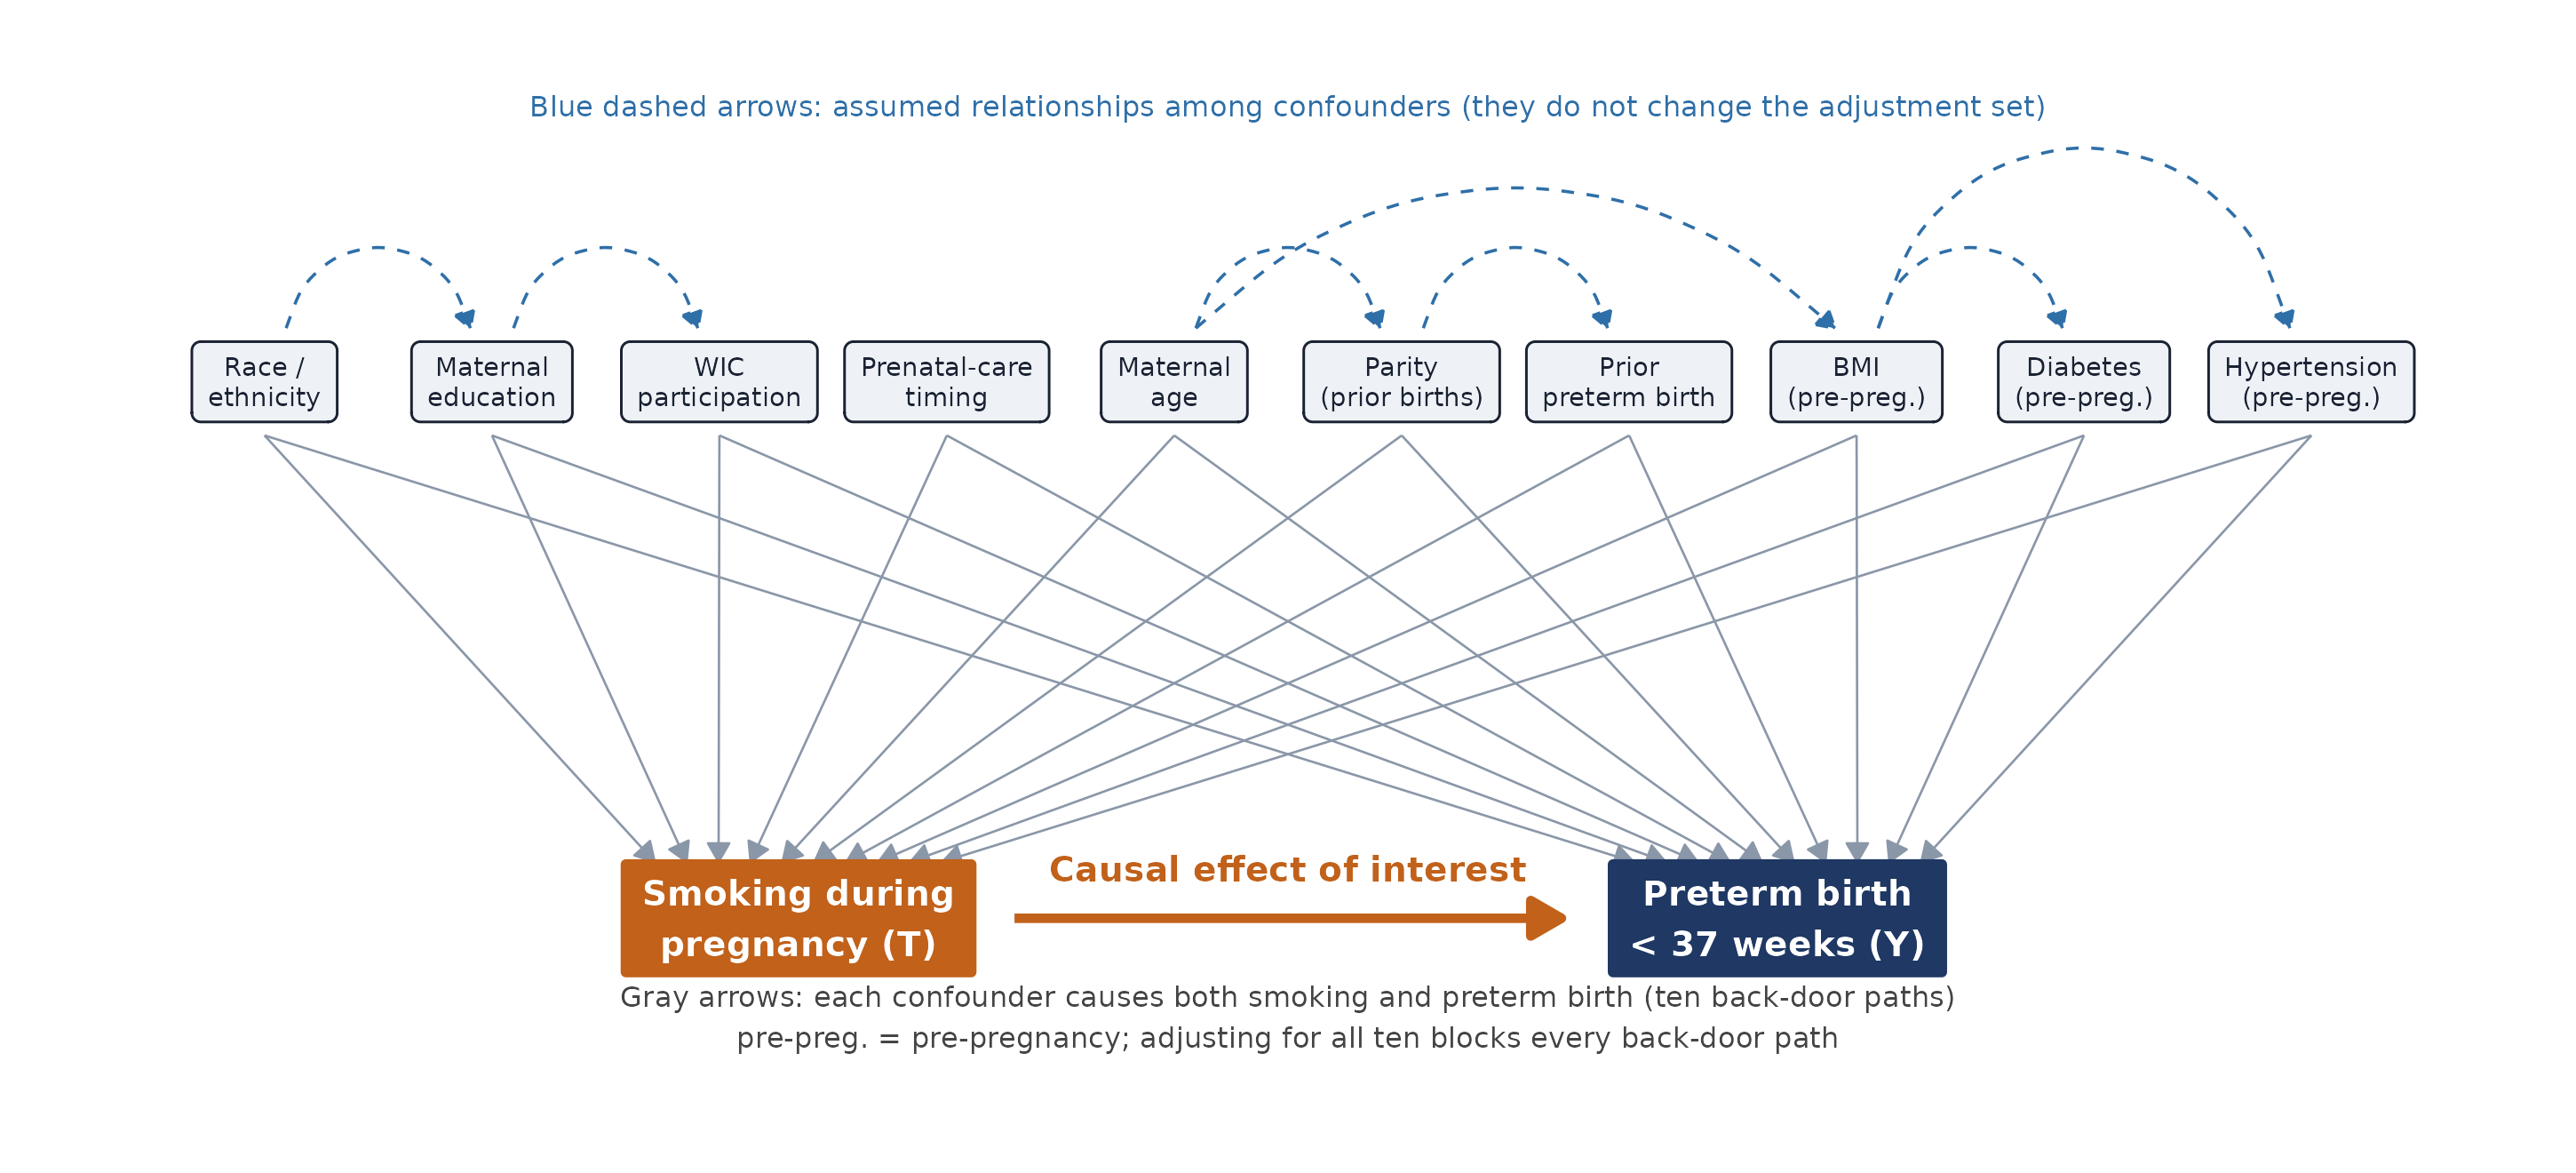
\includegraphics[width=6.2in]{fig_dag.png}
\caption*{\textbf{Figure 1.} \emph{Causal diagram. Orange: exposure ($T$). Navy: outcome ($Y$). Each confounder is a parent of both; dashed blue arrows are assumed relationships among confounders.}}
\end{figure}

\section*{3. Methods}

\textbf{Estimand.} With potential outcomes $Y(1)$ and $Y(0)$, the average treatment effect is $\mathrm{ATE}=\mathbb{E}[Y(1)]-\mathbb{E}[Y(0)]$, the difference in preterm risk if every mother smoked against if none did. The average effect among mothers who smoked (ATT) answers the question for the group exposed. Identification requires conditional exchangeability given the ten confounders, positivity and consistency.

\textbf{AIPTW.} Let $e(X)=P(T=1\mid X)$ and $\mu_t(X)=P(Y=1\mid T=t,X)$. The estimator is
\begin{equation}
\hat\psi_t=\frac1n\sum_{i=1}^{n}\left[\hat\mu_t(X_i)+\frac{\mathbb{1}(T_i=t)\,\big(Y_i-\hat\mu_t(X_i)\big)}{\hat P(T_i=t\mid X_i)}\right],\qquad \widehat{\mathrm{ATE}}=\hat\psi_1-\hat\psi_0 .
\end{equation}
The main analysis uses logistic regression for both models and clamps $\hat e$ at its 1st and 99th percentiles (Funk et al., 2011). Stabilized inverse probability weighting, outcome regression and overlap weights (Li et al., 2018) are reported alongside.

\textbf{Variance.} The standard error is the empirical standard deviation of the estimated influence function divided by $\sqrt n$. It was compared with a full-sample bootstrap in which the propensity model, both outcome models and the estimator were refitted on each of \BootB{} resamples. Because the data collapse to 65,787 covariate cells, resampling the cell counts multinomially is equivalent to resampling births.

\textbf{Flexible nuisance models.} The propensity and outcome models were also fitted by LASSO with all two-way interactions (3-fold cross-validated penalty) and by random forests, each with 5-fold cross-fitting, so that every birth is scored by a model that did not see it (Chernozhukov et al., 2018; Zivich \& Breskin, 2021). The split was repeated \CFreps{} times with different seeds. Calibration of predicted against observed risk was checked for each learner.

\textbf{Overlap and balance.} Standardized mean differences (SMD) were computed for every covariate level before and after weighting; $|{\rm SMD}|>0.10$ was treated as imbalance (Austin \& Stuart, 2015).

\textbf{Smoking history.} The extract records cigarettes per day before pregnancy. Mothers who smoked before but not during pregnancy ("quit") were compared with those who continued, and with those who never smoked. Among those who continued, the effect was estimated by pre-pregnancy intensity. These comparisons are exploratory because intensity during pregnancy and trimester are not in the extract. Timing was studied separately in the full natality file, where the cohort was rebuilt with the same rules and the effect among those who smoked was estimated for four trimester patterns, each against mothers who never smoked, and by third-trimester cigarettes per day among mothers who smoked throughout.

\textbf{Sensitivity.} The risk difference was re-estimated without clamping, with clamping at 0.1/99.9 and 5/95 percentiles, after deleting births with scores outside 0.01 to 0.99, without prenatal-care timing and WIC, with insurance type added, and with two-way interactions. The E-value is $\mathrm{RR}+\sqrt{\mathrm{RR}(\mathrm{RR}-1)}$ (VanderWeele \& Ding, 2017), and measured confounders were used as benchmarks.

\textbf{Software.} All analyses used R with a fixed seed (1234). One script, \texttt{Smoking\_Preterm\_Full\_Analysis.R}, produces every number and figure.

\section*{4. Results}

\textbf{Unadjusted comparison.} Preterm birth occurred in \PretermSmk{}\% of mothers who smoked and \PretermNon{}\% of those who did not, a crude risk difference of \CrudeRD{} points (\CrudeLo{} to \CrudeHi{}) (Figure 2). Smoking was concentrated in specific groups: \SmkNoDip{}\% of mothers with 9 to 12 years of schooling and no diploma smoked, against \SmkDoc{}\% of those with a doctorate.

\begin{figure}[htbp]
\centering
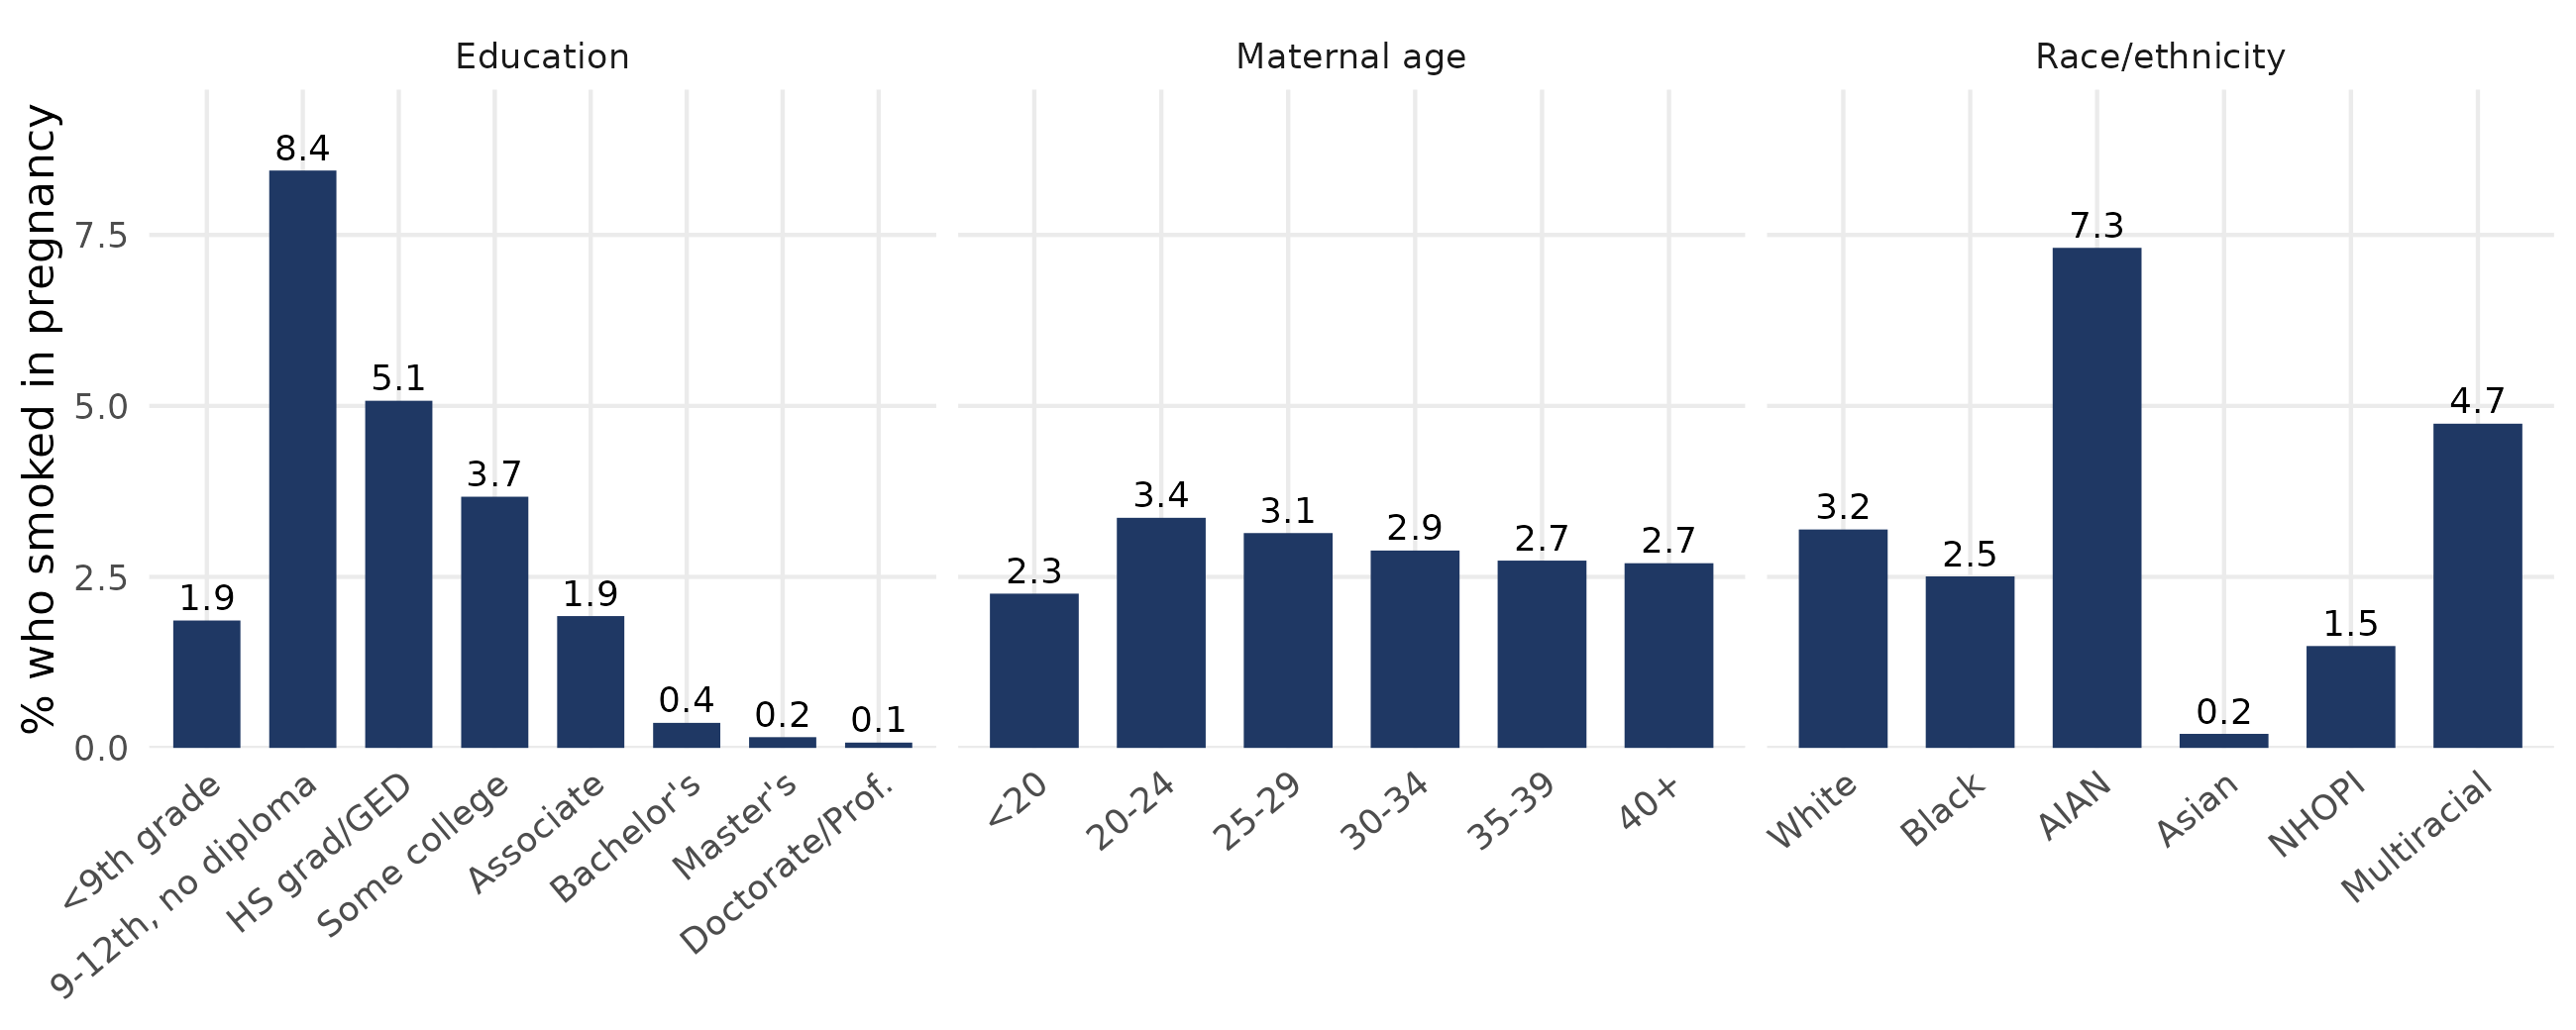
\includegraphics[width=\textwidth]{fig_eda_who_smokes.png}
\caption*{\textbf{Figure 2.} \emph{Percentage of mothers who smoked during pregnancy by education, age and race and ethnicity.}}
\end{figure}

\textbf{Main estimate.} After AIPTW adjustment the risk difference was \RDmain{} points (bootstrap 95\% CI \BootLo{} to \BootHi{}), a risk ratio of \RRmain{} (Table 1, Figure 3). Adjustment reduced the crude difference by \ReducePct{}\%. Outcome regression gave \RDg{} and stabilized IPTW \RDiptw{} (\RDiptwLo{} to \RDiptwHi{}). Among mothers who smoked, the effect was \ATT{} points (\ATTlo{} to \ATThi{}), about \ExcessPerK{} additional preterm births per 1,000 smoking pregnancies or \ExcessBirths{} births in this cohort if the assumptions hold.

\begin{table}[htbp]
\centering
\caption*{\textbf{Table 1.} \emph{Effect of smoking during pregnancy on preterm birth. Risk difference in percentage points. Intervals are from the influence function; the bootstrap interval for the AIPTW estimate is \BootLo{} to \BootHi{}.}}
{\small
\begin{tabular}{lrrr}
\toprule
Estimator & Risk difference (points) & 95\% CI & Risk ratio \\
\midrule
Crude (unadjusted) & 5.60 & 5.38 to 5.82 & 1.68 \\
Outcome regression (g-computation) & 3.48 &  &  \\
IPTW (stabilized) & 3.53 & 2.77 to 4.30 & 1.42 \\
AIPTW (doubly robust) & 3.26 & 2.47 to 4.04 & 1.39 \\
AIPTW, effect among smokers (ATT) & 3.39 & 3.17 to 3.61 &  \\
Overlap weights (ATO) & 3.30 & 3.08 to 3.52 & 1.32 \\
\bottomrule
\end{tabular}
}

\end{table}

\begin{figure}[htbp]
\centering
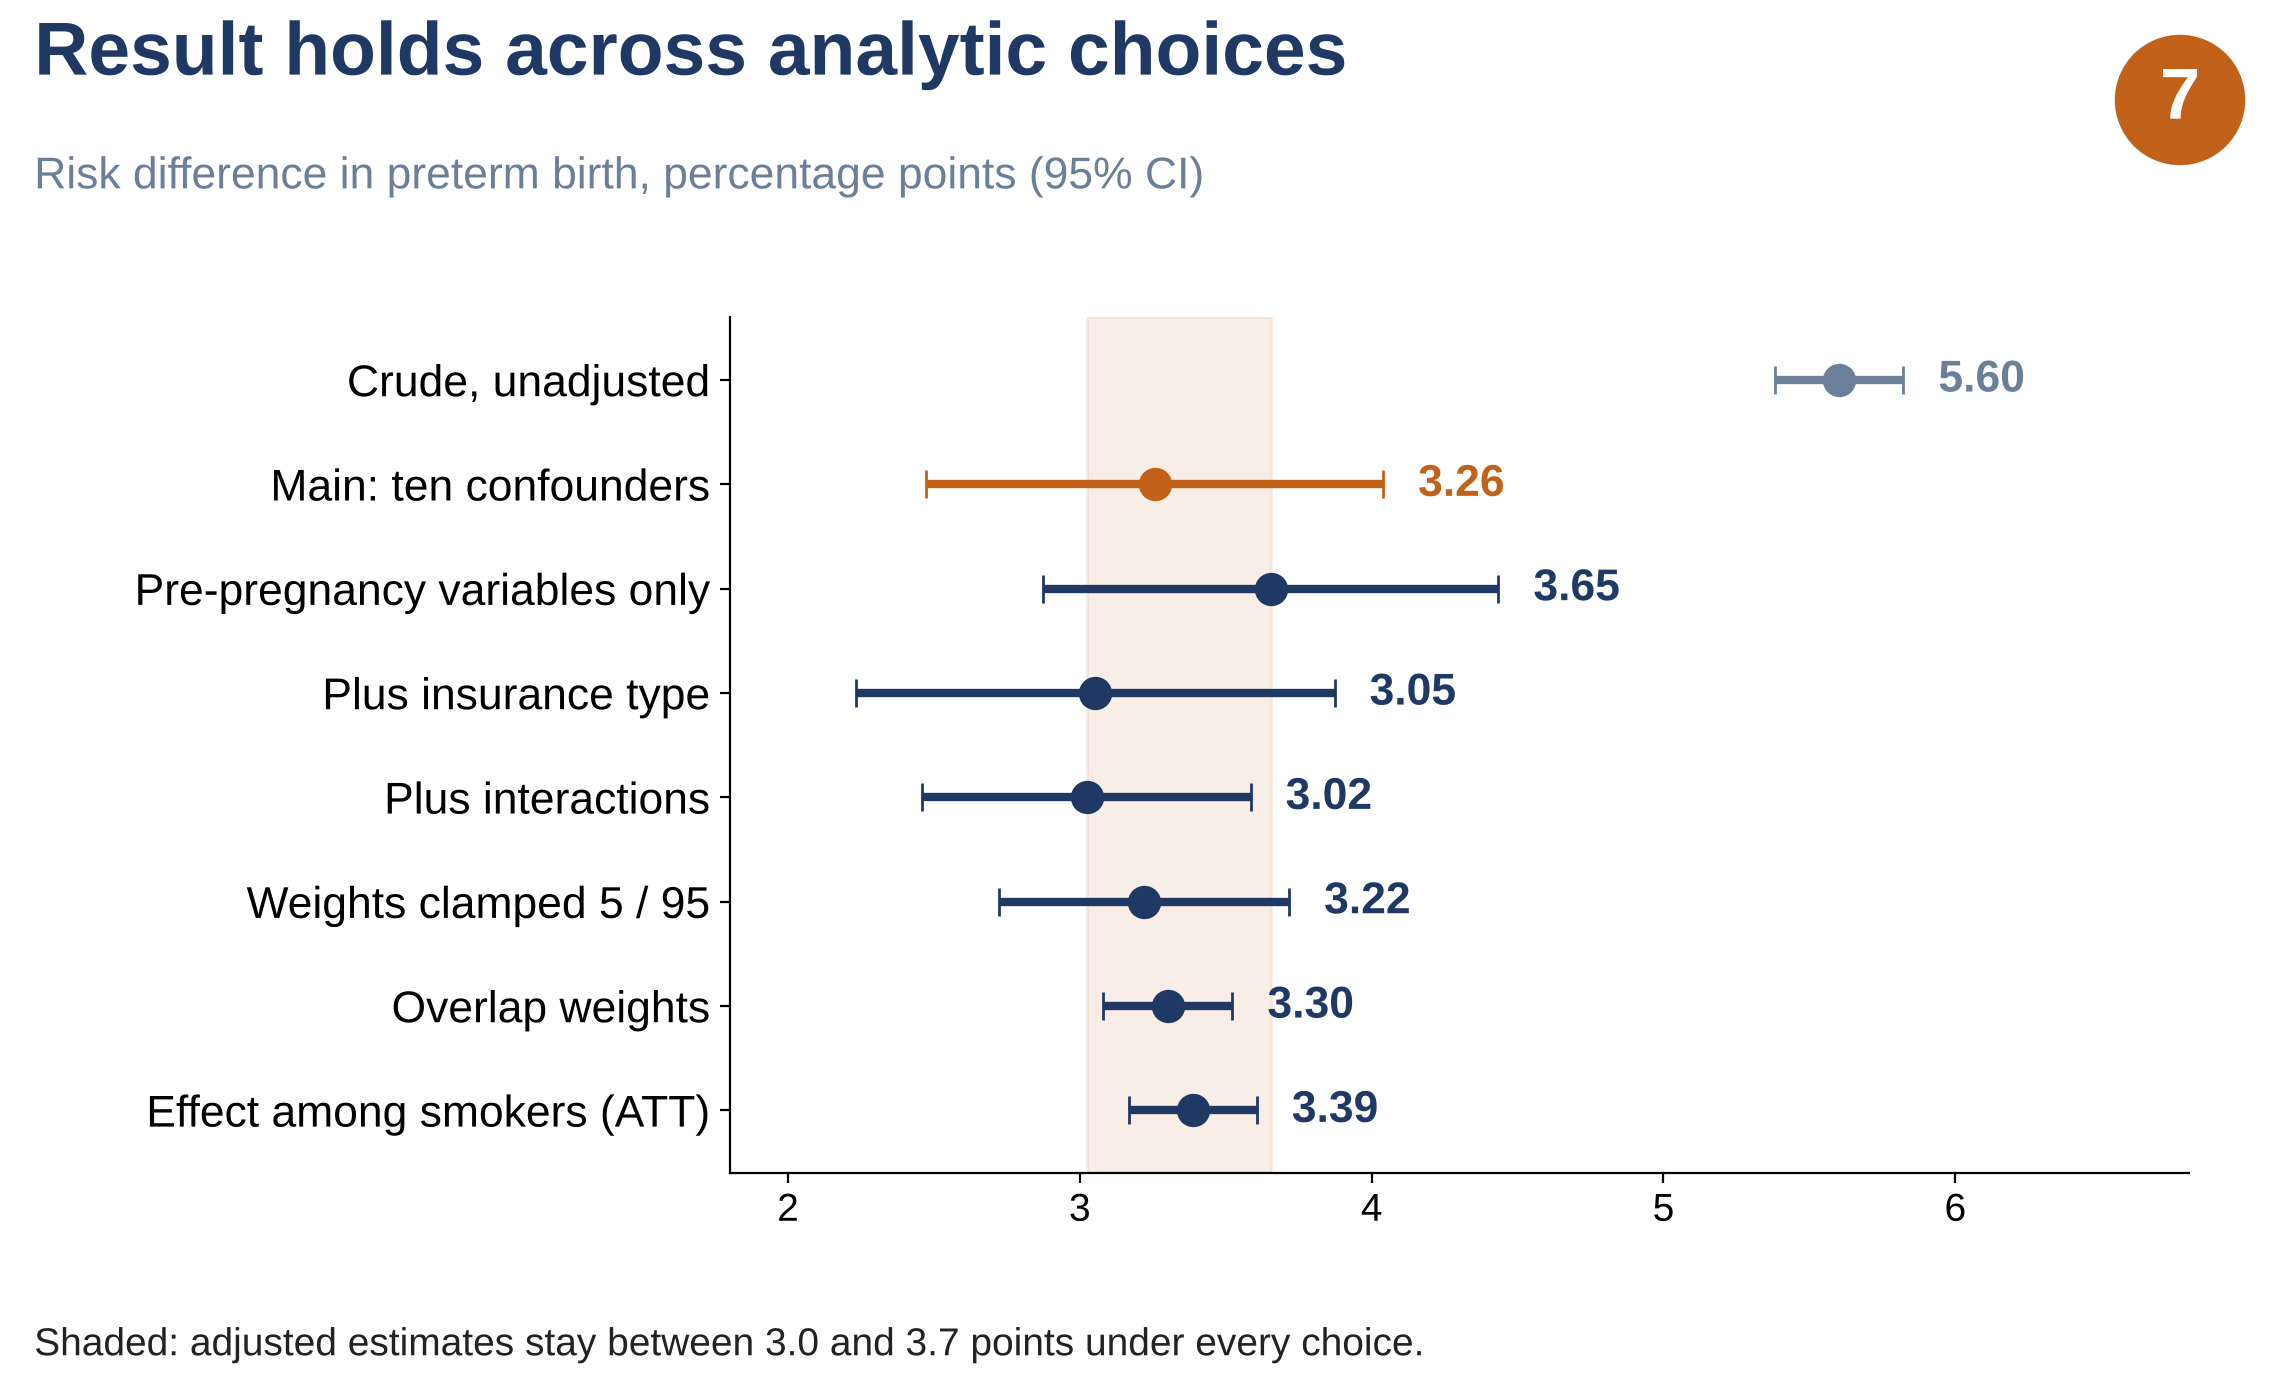
\includegraphics[width=5.8in]{f7_robust.png}
\caption*{\textbf{Figure 3.} \emph{Risk difference under alternative propensity score handling and covariate sets.}}
\end{figure}

\textbf{Robustness to model and specification choices.} The risk difference ranged from \RangeMin{} to \RangeMax{} points across all specifications (Table 2). Removing prenatal-care timing and WIC gave \RDPre{} (\RDPreLo{} to \RDPreHi{}), a shift of \PreShift{} points, the largest change among the specifications examined. Without any clamping the estimate was \RDnoclamp{}, with a largest weight of \MaxWtNone{}, against \MaxWtClamp{} with clamping.

\begin{table}[htbp]
\centering
\caption*{\textbf{Table 2.} \emph{AIPTW risk difference under alternative covariate sets and propensity score rules.}}
{\small
\begin{tabular}{lrr}
\toprule
Analysis & Risk difference (points) & 95\% CI \\
\midrule
Crude, unadjusted & 5.60 & 5.38 to 5.82 \\
Main: ten confounders & 3.26 & 2.47 to 4.04 \\
Pre-pregnancy set only (no care timing, no WIC) & 3.65 & 2.88 to 4.43 \\
Main plus insurance type & 3.05 & 2.23 to 3.87 \\
Main plus two-way interactions & 3.02 & 2.46 to 3.59 \\
Clamp at 5 / 95 percentile & 3.22 & 2.72 to 3.72 \\
Overlap weights & 3.30 & 3.08 to 3.52 \\
Among smokers (ATT) & 3.39 & 3.17 to 3.61 \\
\bottomrule
\end{tabular}
}

\end{table}

\textbf{Overlap and balance.} The propensity score separated the groups only partly (Figure 4). \LowNon{}\% of non-smokers, but \LowSmk{}\% of smokers, had a score below 0.01, and \LowBachSum{}\% of the non-smokers in that low group held a bachelor's degree or higher, the group in which smoking is rare. The largest SMD fell from \SMDbefore{} before weighting to \SMDafter{} after IPTW (\BalAfter{} of \NLevels{} levels above 0.10, down from \BalBefore{}) and to \SMDov{} with overlap weights. The largest stabilized weight among smokers was \MaxWtClamp{} and the effective sample size of the weighted smokers was \ESSclamp{} of \NSmokers{}.

\begin{figure}[htbp]
\centering
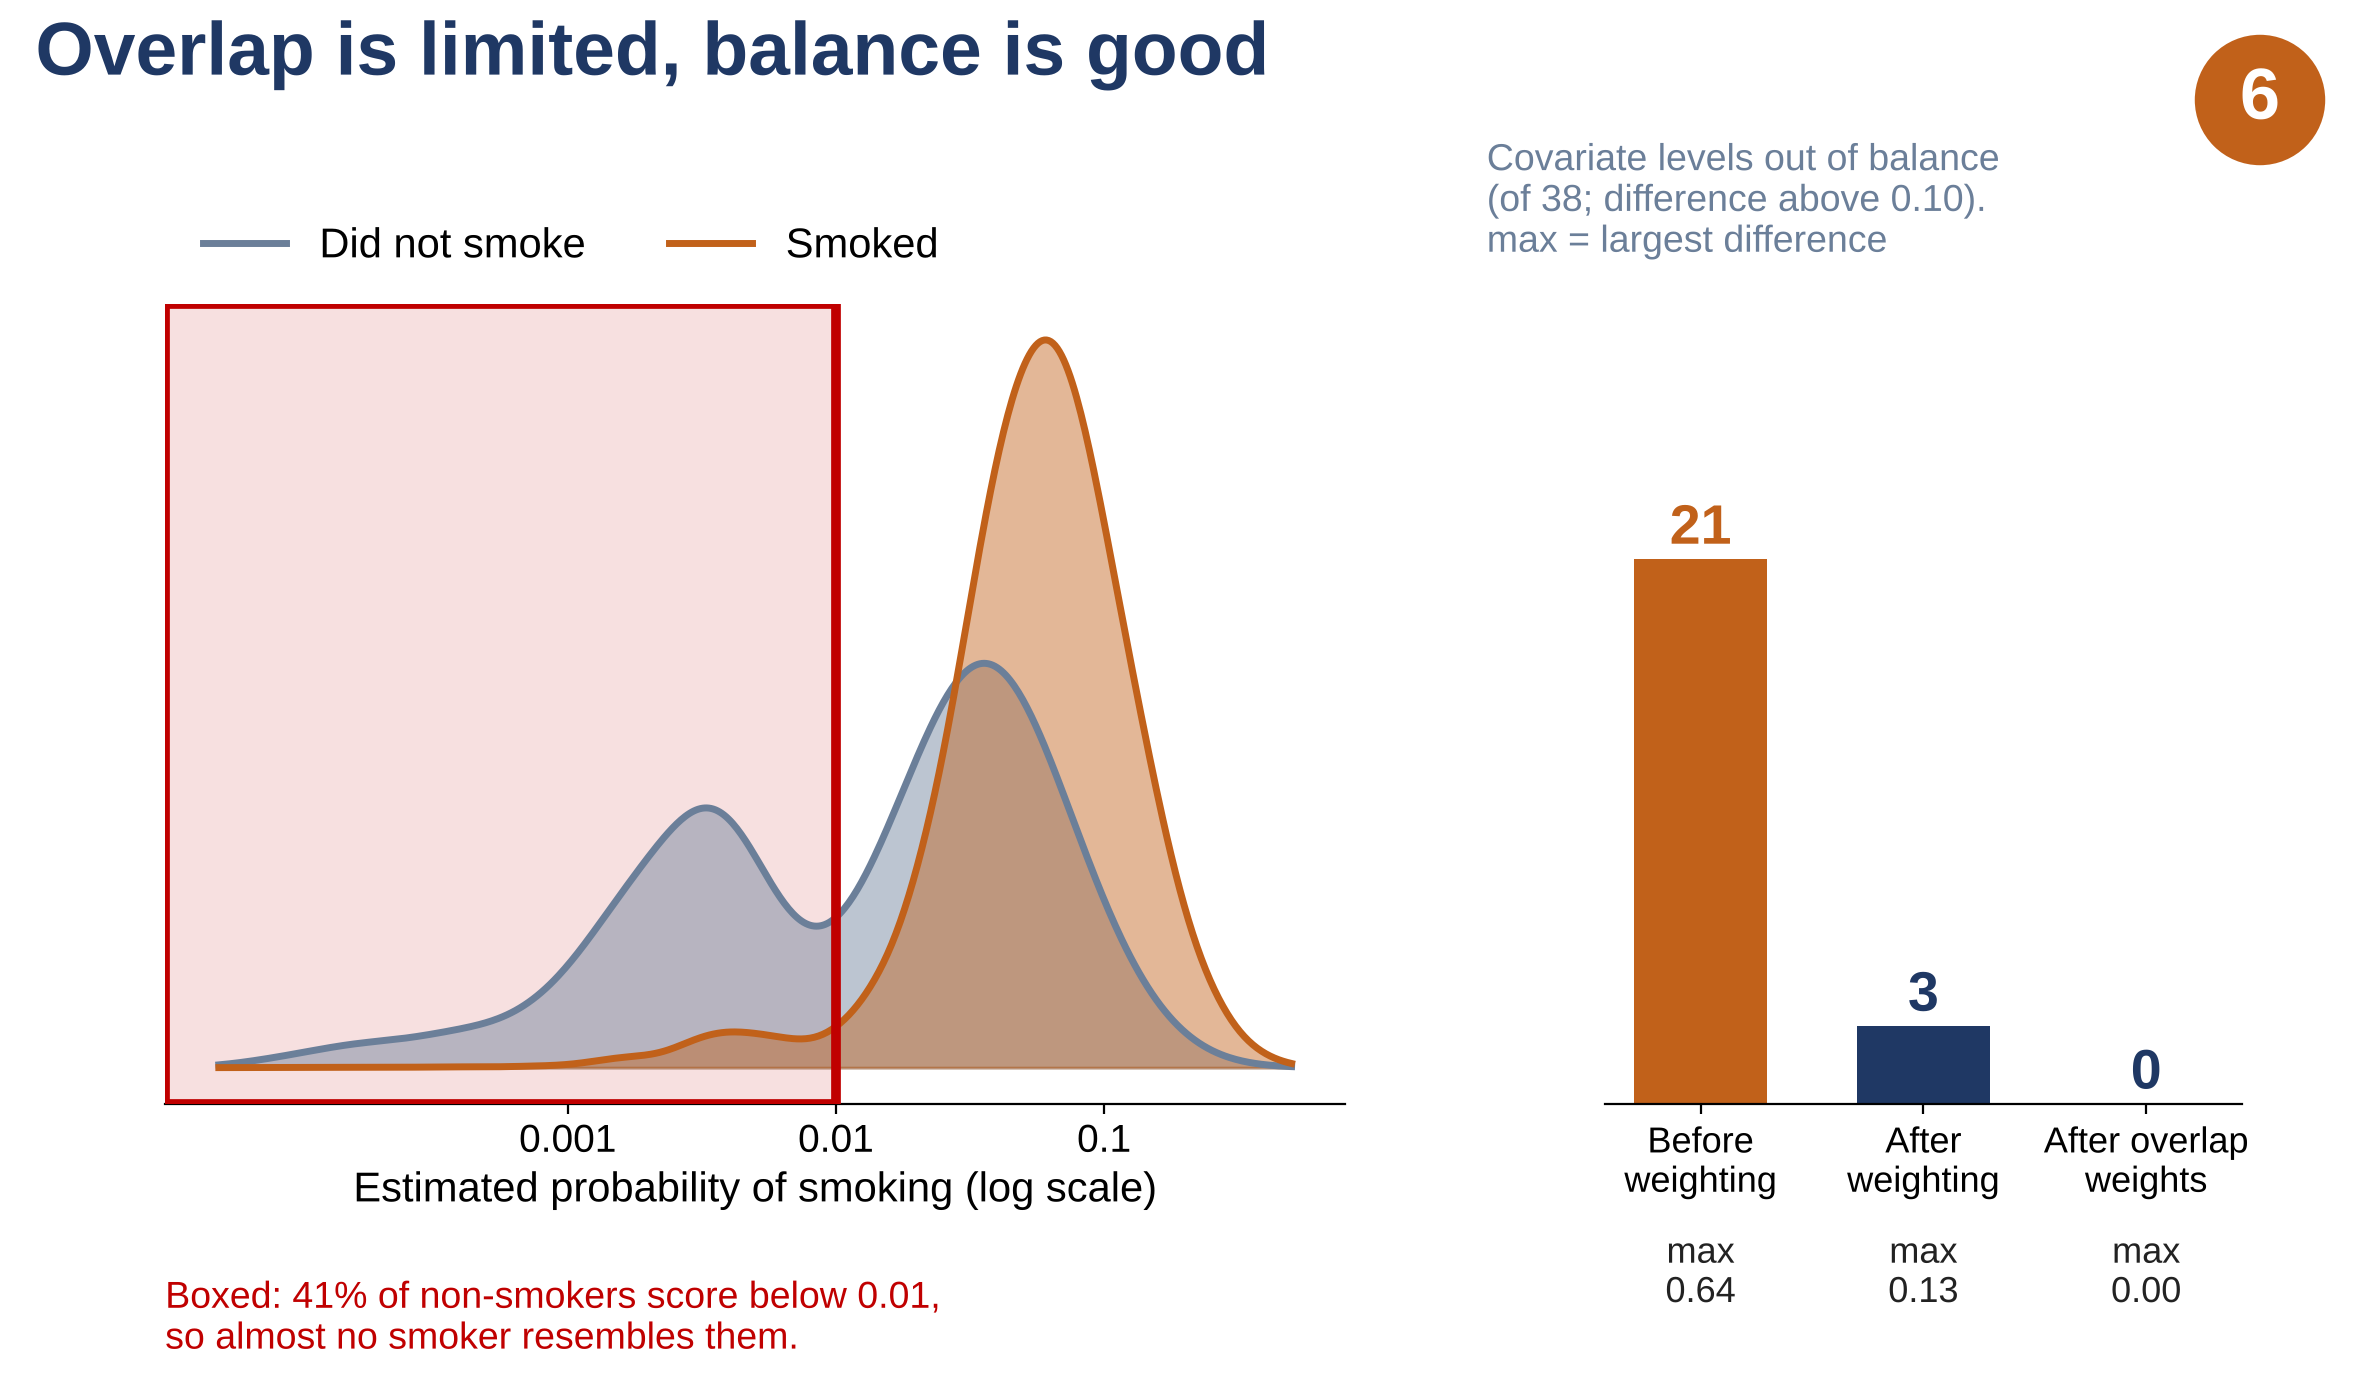
\includegraphics[width=\textwidth]{f6_overlap.png}
\caption*{\textbf{Figure 4.} \emph{Estimated probability of smoking by smoking status, with the share of non-smokers below 0.01 and covariate balance before and after weighting.}}
\end{figure}

\textbf{Variance.} The bootstrap standard error was \SEboot{} points (percentile 95\% CI \BootLo{} to \BootHi{}) against \SEif{} from the influence function, a ratio of \SEratio{} (Appendix Table A3). The two standard errors are nearly identical, so the influence-function standard error is reliable here; the bootstrap percentile interval is reported as the primary interval.

\textbf{Flexible models.} With cross-fitting, the risk difference was \CFLog{} with logistic regression, \CFLasso{} with LASSO and \CFForest{} with random forests; the average of the three was \CFAvg{} (Table 3, Figure 5). The 95\% intervals overlap those of the main estimate. Calibration of each learner is reported in Appendix Table A4.

\begin{table}[htbp]
\centering
\caption*{\textbf{Table 3.} \emph{Cross-fitted AIPTW with three learners (clamped at 1/99 percentiles).}}
\resizebox{\textwidth}{!}{{\small
\begin{tabular}{lrrrrrr}
\toprule
Learner & Risk difference & 95\% CI & Outcome part & Weighting part & Largest weight & Effective n \\
\midrule
Logistic, main effects & 3.22 & 2.43 to 4.01 & 3.48 & 3.52 & 6,308 & 6,755 \\
LASSO with all two-way interactions & 2.80 & 2.02 to 3.57 & 3.85 & 3.01 & 6,922 & 6,428 \\
Random forest & 2.30 & 1.39 to 3.21 & 3.77 & 2.51 & 10,000 & 3,788 \\
Average of the three & 2.84 & 2.28 to 3.41 & 3.70 & 3.00 & 4,594 & 8,808 \\
\bottomrule
\end{tabular}
}
}
\end{table}

\begin{figure}[htbp]
\centering
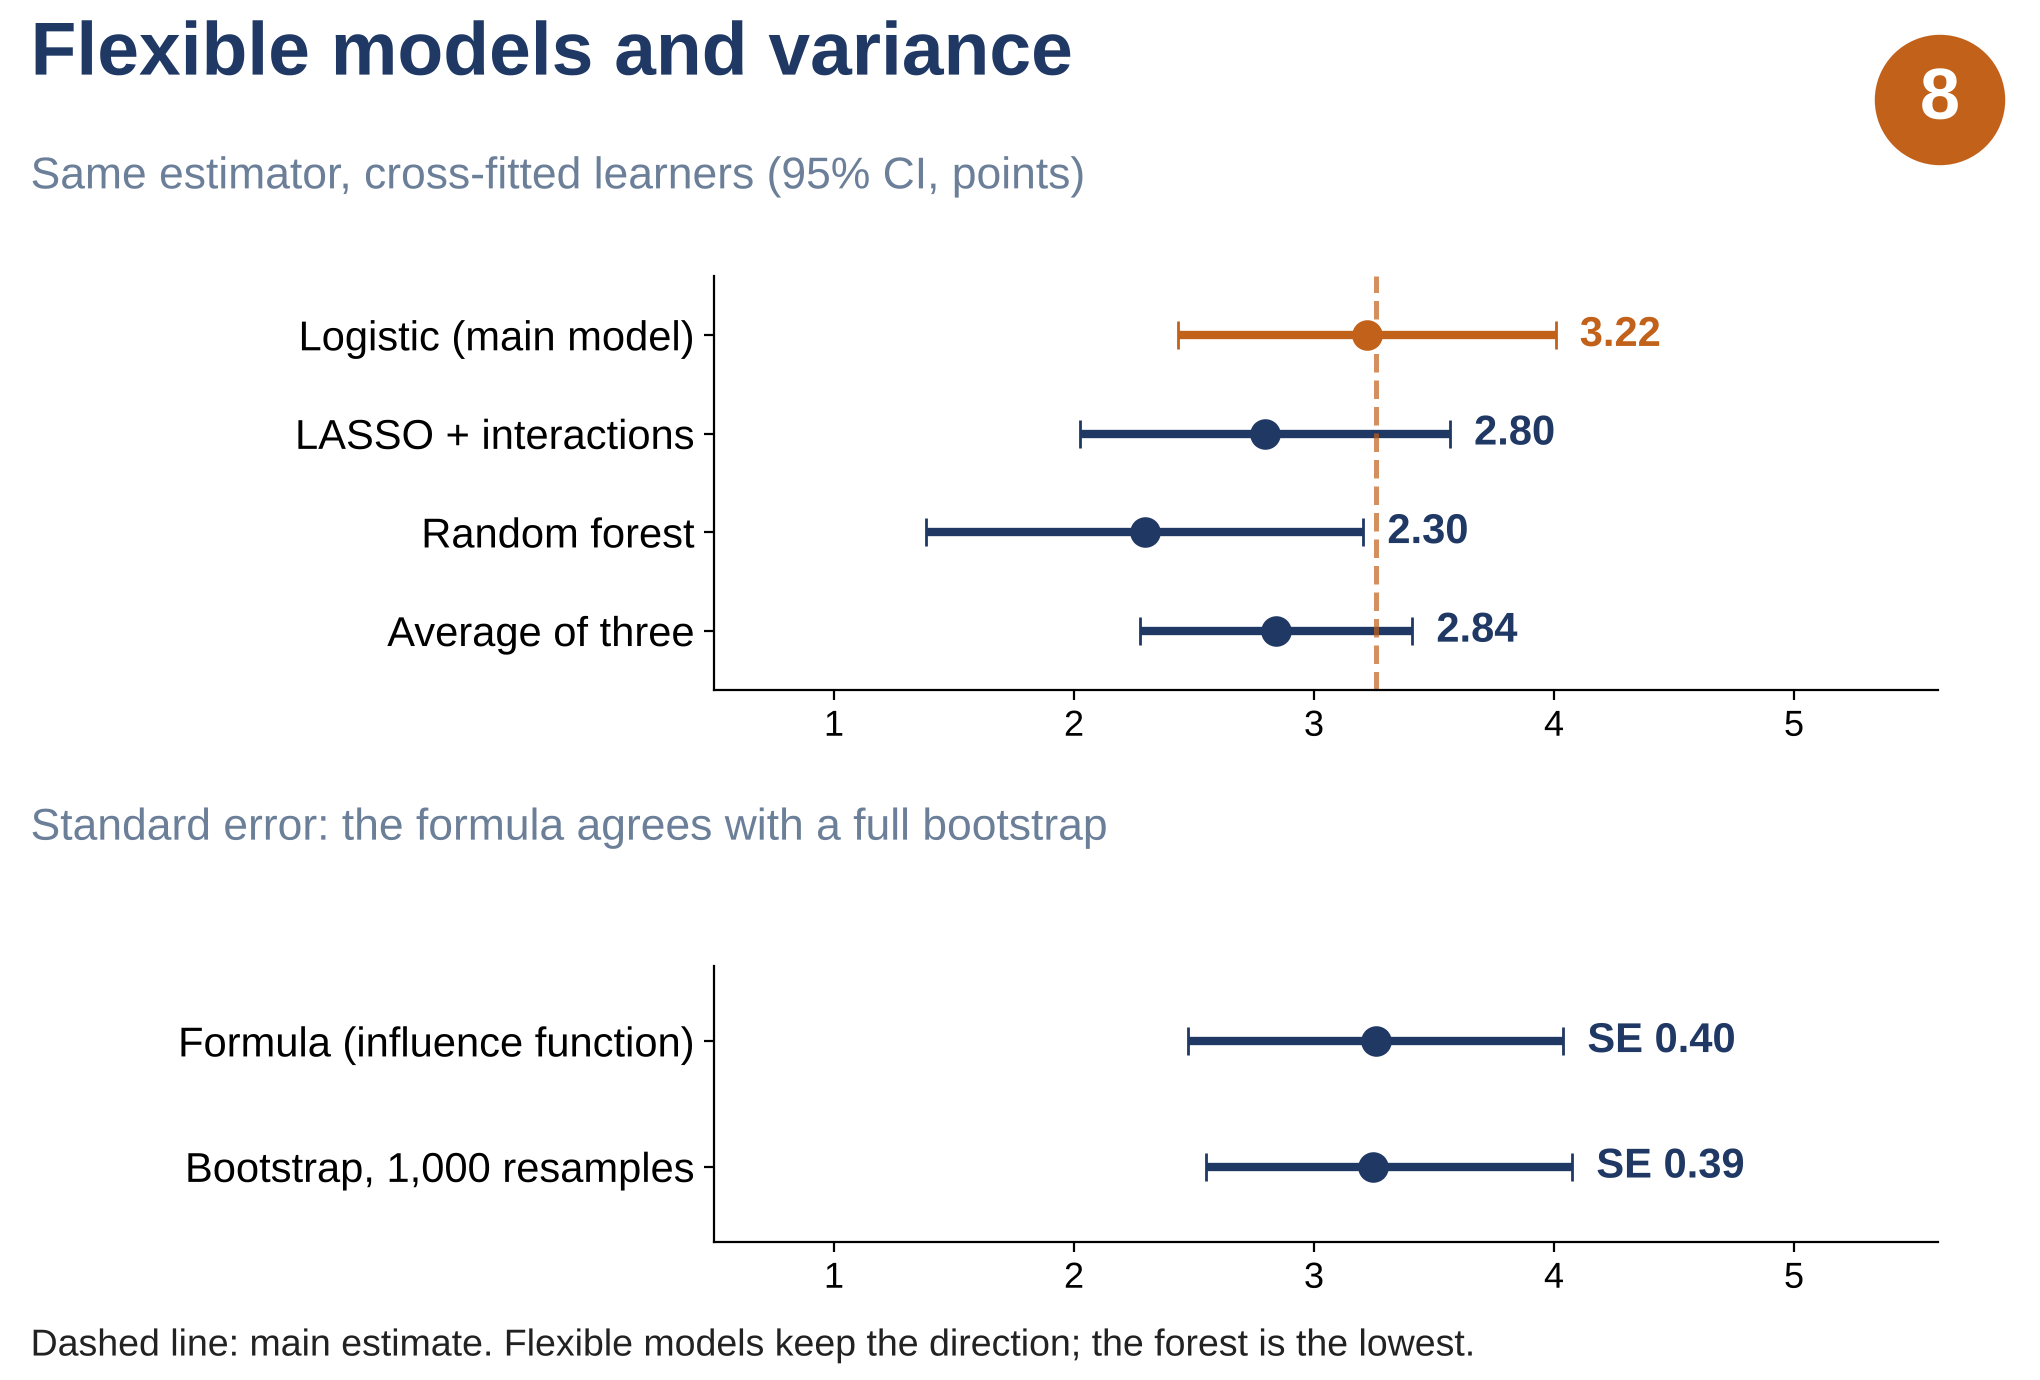
\includegraphics[width=\textwidth]{f8_flex.png}
\caption*{\textbf{Figure 5.} \emph{Cross-fitted estimates by learner, and influence-function against bootstrap standard errors.}}
\end{figure}

\textbf{Smoking history and intensity (exploratory).} Crude preterm risk was \HistNever{}\% in mothers who never smoked, \HistQuit{}\% in those who quit, \HistCont{}\% in those who continued and \HistStart{}\% in those who started during pregnancy (Appendix Table A5). Comparing continuers with quitters, adjusted for the confounders and pre-pregnancy intensity, gave \ContQuit{} points (\ContQuitLo{} to \ContQuitHi{}). Quitters compared with never-smokers differed by \QuitNever{} points among quitters (\QuitNeverLo{} to \QuitNeverHi{}) and by \QuitNeverATE{} points in the whole population (Figure 6).

\begin{figure}[htbp]
\centering
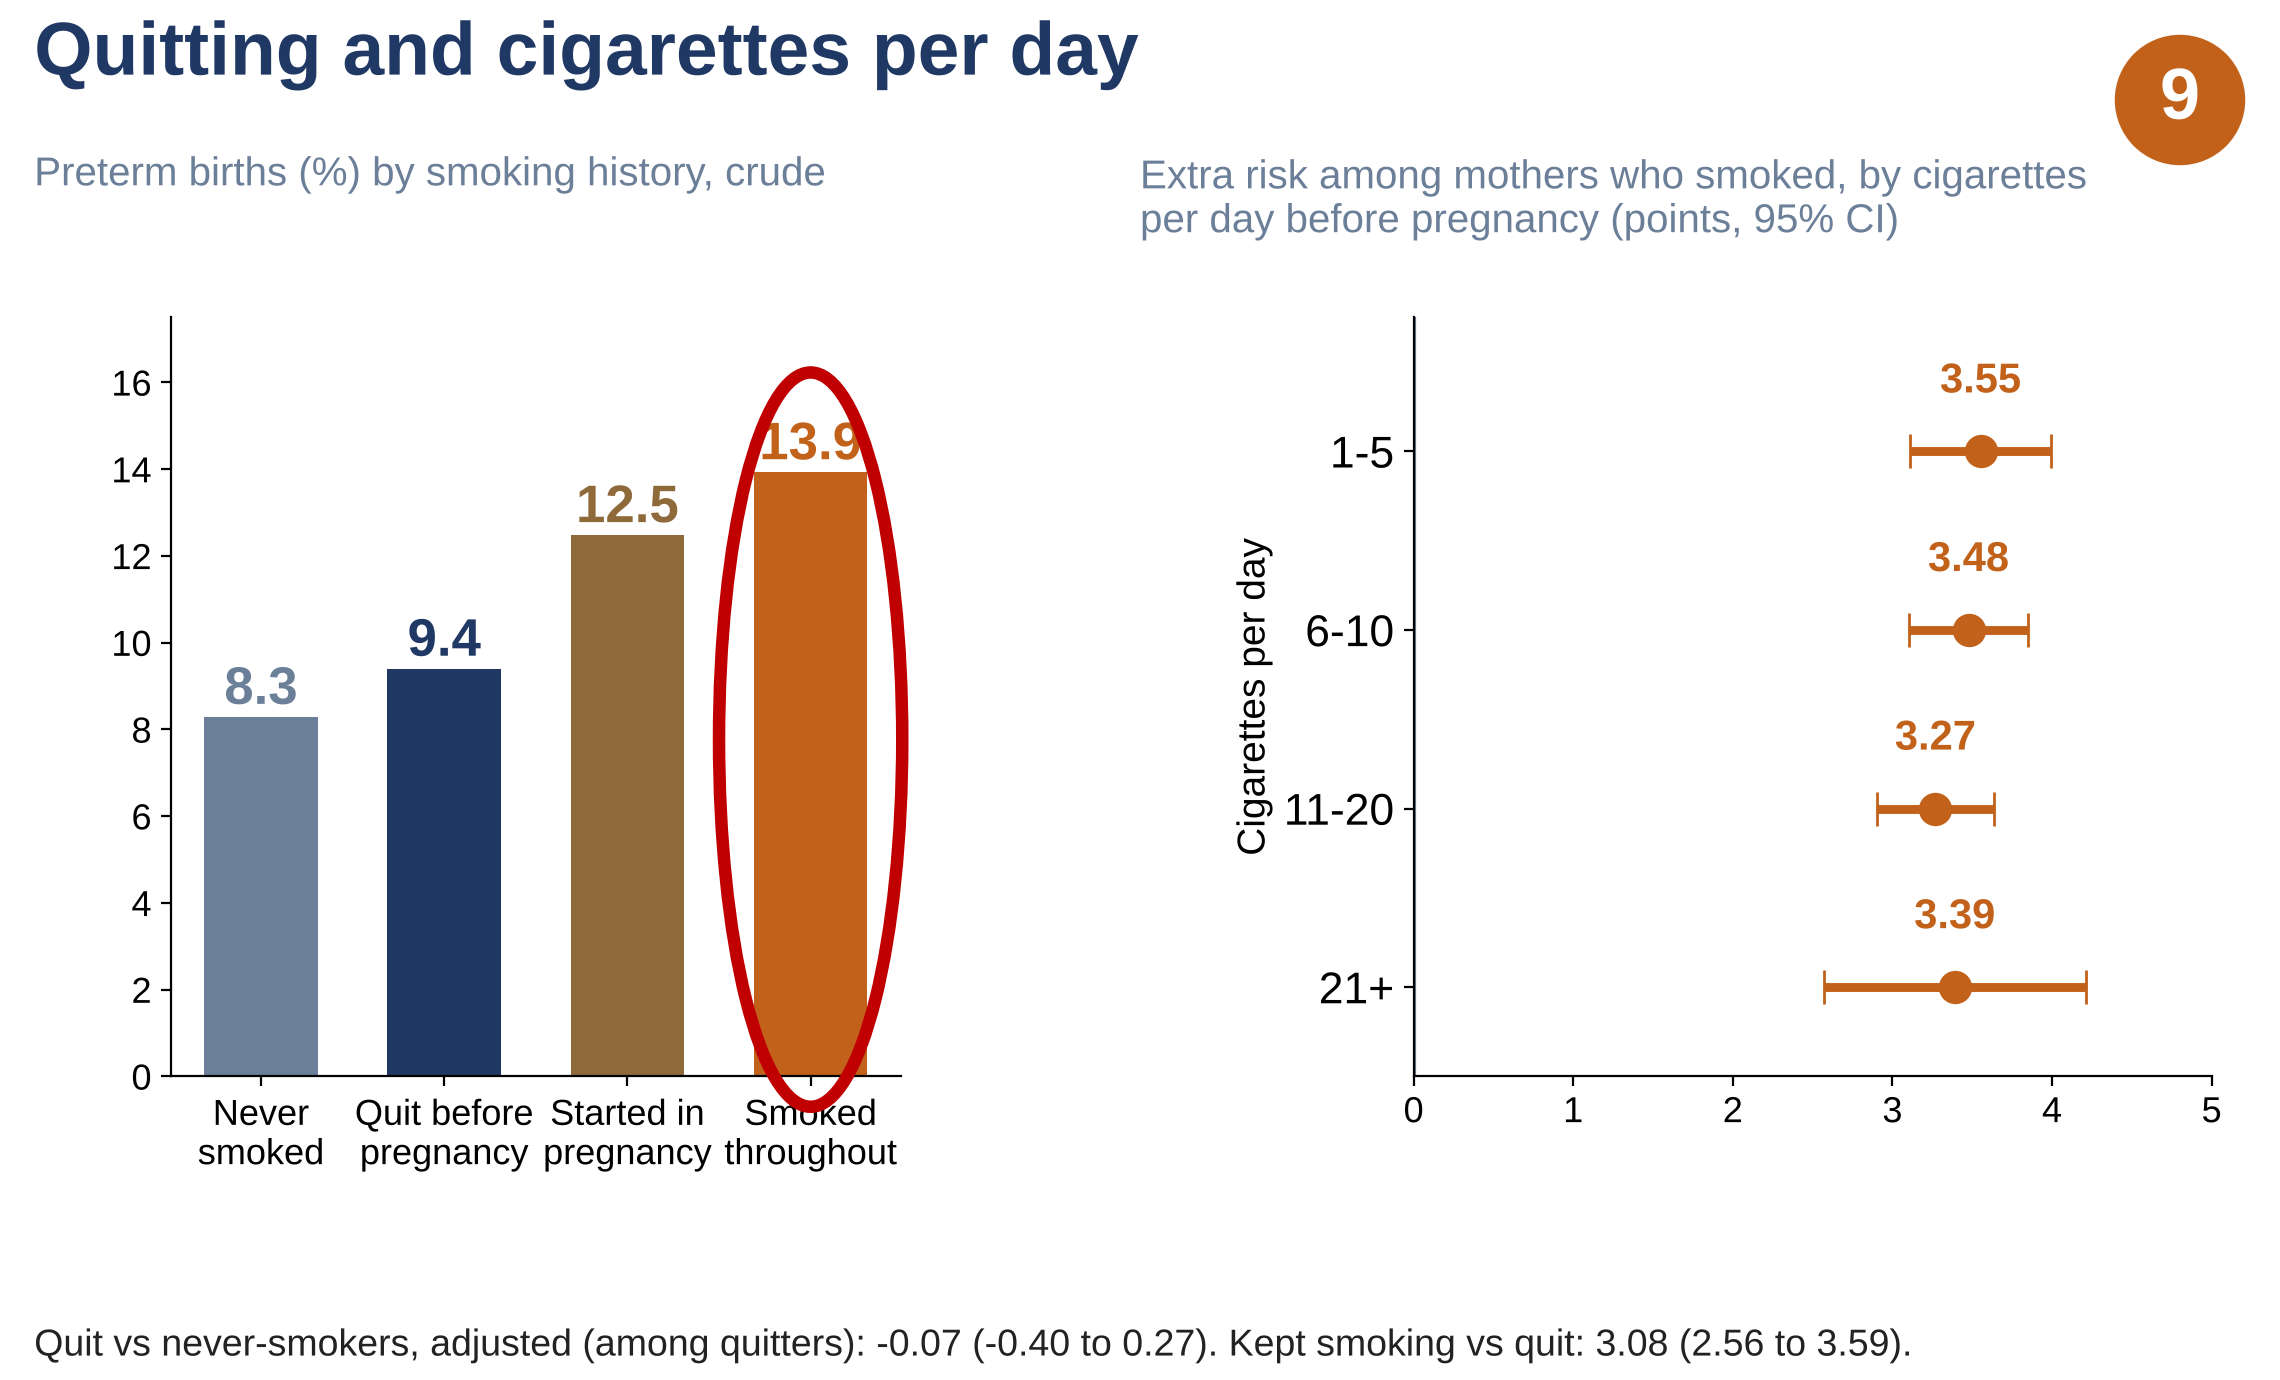
\includegraphics[width=\textwidth]{f9_cess.png}
\caption*{\textbf{Figure 6.} \emph{Effect among those who smoked by smoking history and by pre-pregnancy cigarettes per day.}}
\end{figure}

\textbf{Timing of smoking by trimester (exploratory).} The full 2023 natality file records cigarettes per day in each trimester, which the extract does not. Rebuilding the cohort from the full file gave the same \NTotal{} births, and \TriN{} of them had known cigarettes in every period. Mothers were grouped by the trimesters in which they smoked and each group was compared with mothers who smoked in no period, before or during pregnancy (Appendix Table A7). Crude preterm risk was \TriNever{}\% in the reference group, \TriFirst{}\% in mothers who smoked in the first trimester only, \TriFirstSecond{}\% in the first and second trimesters only, \TriAll{}\% in all three trimesters and \TriLate{}\% in those who started after the first trimester. After adjustment, the effect among those who smoked was \TriAATT{} points (\TriALo{} to \TriAHi{}) for the first trimester only, \TriBATT{} (\TriBLo{} to \TriBHi{}) for the first and second trimesters and \TriCATT{} (\TriCLo{} to \TriCHi{}) for all three. The \TriLateN{} mothers who started after the first trimester gave \TriDATT{} points (\TriDLo{} to \TriDHi{}), too imprecise to read. Among mothers who smoked in all three trimesters the effect rose with third-trimester intensity: \TriDoseA{}, \TriDoseB{}, \TriDoseC{} and \TriDoseD{} points at 1 to 5, 6 to 10, 11 to 20 and 21 or more cigarettes per day. As in the pre-pregnancy intensity analysis, the whole-population estimate for the smallest group is unstable (\TriDoseWideATE{} points, \TriDoseWideLo{} to \TriDoseWideHi{} for 21 or more), so the effect among smokers is the reading to use. The time a mother can smoke is limited by when she delivers, so the shorter-exposure groups contain early deliveries by construction, and these comparisons describe patterns of reported smoking rather than the effect of stopping at a chosen time.

\textbf{Unmeasured confounding.} The E-value for the point estimate was \EV{} and for the lower confidence limit \EVlo{}. Previous preterm birth, the strongest measured predictor of preterm birth, changed the estimate by \PPChange{} points when left out and education by \EducChange{} points; previous preterm birth is the only measured level whose association with both smoking (risk ratio 2.42) and preterm birth (3.42) exceeds the E-value, and omitting it moves the estimate by only \PPChange{} points (Appendix Table A6).

\section*{5. Discussion}

In 2023 U.S. singleton births, smoking during pregnancy raised the risk of preterm birth by about \RDmain{} percentage points (risk ratio \RRmain{}) under the stated assumptions, which is \ReducePct{}\% less than the crude difference. The adjusted marginal odds ratio of 1.44 lies inside the 1.31 to 1.53 range reported for first-trimester smoking by cigarettes per day in a regression analysis of 25.6 million births (Liu et al., 2020). Among mothers who smoked, the effect translates to about \OneIn{} smoking pregnancies for each additional preterm birth, which gives health departments a count to use when comparing cessation programs.

Four findings support the stability of the result. The standard error did not change materially when the whole pipeline was resampled. The estimate moved little when the nuisance models were flexible and cross-fitted. It stayed within \RangeMin{} to \RangeMax{} points across specifications. And the overlap-weighted estimate, which targets mothers with comparable counterparts, was \ATO{} points. The effect among smokers was smaller for mothers who smoked only in the first trimester (\TriAATT{} points) than for those who smoked in all three (\TriCATT{} points), in line with a benefit of stopping early. The exposure-history comparison is also consistent with a benefit of stopping smoking, but both analyses are exploratory and was adjusted only for the covariates and pre-pregnancy intensity in the extract.

\section*{6. Limitations}

Smoking is self-reported on the birth certificate and is underreported (Dietz et al., 2011; Howland et al., 2015; Searles Nielsen et al., 2014). Non-differential misclassification of a binary exposure usually biases toward the null (Jurek et al., 2005). Overlap is limited: \LowNon{}\% of non-smokers have a score below 0.01, concentrated among mothers with a college degree, so the ATE depends on few smokers with large weights. The ATT, which needs weights only for non-smokers, and the overlap-weighted estimate are less affected. Prenatal-care timing and WIC may follow smoking, and the estimate without them was \RDPre{}. Complete-case analysis excluded \NDropped{} births, whose preterm risk was higher (\DroppedPreterm{}\% against \KeptPreterm{}\%). The file contains live births only (Leung et al., 2021). Alcohol, cannabis, e-cigarettes, stress and interpregnancy interval are unmeasured (Patra et al., 2011; Regan et al., 2021). ``Any smoking'' averages over dose and timing. Intensity during pregnancy and trimester of smoking are not in the 24-variable extract; they are in the full natality file and are analysed in the trimester section. The results are for one national year.

\section*{7. Conclusion}

In \NTotal{} singleton births, the AIPTW risk difference for preterm birth was \RDmain{} percentage points (95\% bootstrap CI \BootLo{} to \BootHi{}), \ATT{} points among mothers who smoked. The estimate was stable across bootstrap, flexible learners and specification changes, and it rests on limited overlap, self-reported smoking and assumptions the E-value quantifies but cannot verify.

\section*{Data and code availability}

The data are the public-use 2023 Natality file of the National Center for Health Statistics (\url{https://ftp.cdc.gov/pub/Health_Statistics/NCHS/Datasets/DVS/natality/Nat2023us.zip}). The 24-variable extract and the script \texttt{Smoking\_Preterm\_Full\_Analysis.R} are in the project repository (\url{https://github.com/fmurital/Causal-Inference-}, folder \texttt{3\_Journal\_Paper}); the script reads the extract directly from the repository and runs from one file with seed 1234.

\section*{Use of AI assistance}

The authors used an AI assistant (Claude, Anthropic) to organize the literature, to help write and test the R code, and to draft and edit text. The first author specified the question, the design and the analytic choices and ran the code. The numbers come directly from the code output. Both authors are responsible for the content.

\section*{References}
{\small\setlength{\parindent}{-0.25in}\setlength{\leftskip}{0.25in}\setlength{\parskip}{3pt}
Austin, P. C., \& Stuart, E. A. (2015). Moving towards best practice when using inverse probability of treatment weighting (IPTW) using the propensity score to estimate causal treatment effects in observational studies. Statistics in Medicine, 34(28), 3661-3679. \url{https://doi.org/10.1002/sim.6607}

Bang, H., \& Robins, J. M. (2005). Doubly robust estimation in missing data and causal inference models. Biometrics, 61(4), 962-973. \url{https://doi.org/10.1111/j.1541-0420.2005.00377.x}

Chernozhukov, V., Chetverikov, D., Demirer, M., Duflo, E., Hansen, C., Newey, W., \& Robins, J. (2018). Double/debiased machine learning for treatment and structural parameters. The Econometrics Journal, 21(1), C1-C68. \url{https://doi.org/10.1111/ectj.12097}

Dietz, P. M., Homa, D., England, L. J., Burley, K., Tong, V. T., Dube, S. R., \& Bernert, J. T. (2011). Estimates of nondisclosure of cigarette smoking among pregnant and nonpregnant women of reproductive age in the United States. American Journal of Epidemiology, 173(3), 355-359. \url{https://doi.org/10.1093/aje/kwq381}

Funk, M. J., Westreich, D., Wiesen, C., Stürmer, T., Brookhart, M. A., \& Davidian, M. (2011). Doubly robust estimation of causal effects. American Journal of Epidemiology, 173(7), 761-767. \url{https://doi.org/10.1093/aje/kwq439}

Howland, R. E., Mulready-Ward, C., Madsen, A. M., Sackoff, J., Nyland-Funke, M., Bombard, J. M., \& Tong, V. T. (2015). Reliability of reported maternal smoking: Comparing the birth certificate to maternal worksheets and prenatal and hospital medical records, New York City and Vermont, 2009. Maternal and Child Health Journal, 19(9), 1916-1924. \url{https://doi.org/10.1007/s10995-015-1722-1}

Joyce, T., Racine, A., \& Yunzal-Butler, C. (2008). Reassessing the WIC effect: Evidence from the Pregnancy Nutrition Surveillance System. Journal of Policy Analysis and Management, 27(2), 277-303.

Jurek, A. M., Greenland, S., Maldonado, G., \& Church, T. R. (2005). Proper interpretation of non-differential misclassification effects: Expectations vs observations. International Journal of Epidemiology, 34(3), 680-687. \url{https://doi.org/10.1093/ije/dyi060}

Kondracki, A. J. (2020). Low birthweight in term singletons mediates the association between maternal smoking intensity exposure status and immediate neonatal intensive care unit admission: The E-value assessment. BMC Pregnancy and Childbirth. \url{https://doi.org/10.1186/s12884-020-02981-1}

Leung, M., Kioumourtzoglou, M.-A., Raz, R., \& Weisskopf, M. G. (2021). Bias due to selection on live births in studies of environmental exposures during pregnancy: A simulation study. Environmental Health Perspectives, 129(4), 047001. \url{https://doi.org/10.1289/EHP7961}

Li, F., Morgan, K. L., \& Zaslavsky, A. M. (2018). Balancing covariates via propensity score weighting. Journal of the American Statistical Association, 113(521), 390-400. \url{https://doi.org/10.1080/01621459.2016.1260466}

Liu, B., Xu, G., Sun, Y., Qiu, X., Ryckman, K. K., Yu, Y., Snetselaar, L. G., \& Bao, W. (2020). Maternal cigarette smoking before and during pregnancy and the risk of preterm birth: A dose-response analysis of 25 million mother-infant pairs. PLOS Medicine, 17(8), e1003158. \url{https://doi.org/10.1371/journal.pmed.1003158}

Martin, J. A., Hamilton, B. E., \& Osterman, M. J. K. (2024). Births in the United States, 2023 (NCHS Data Brief No. 507). National Center for Health Statistics. \url{https://doi.org/10.15620/cdc/158789}

Martin, J. A., Osterman, M. J. K., \& Driscoll, A. K. (2023). Declines in cigarette smoking during pregnancy in the United States, 2016-2021 (NCHS Data Brief No. 458). National Center for Health Statistics.

Martin, J. A., Osterman, M. J. K., Kirmeyer, S. E., \& Gregory, E. C. W. (2015). Measuring gestational age in vital statistics data: Transitioning to the obstetric estimate. National Vital Statistics Reports, 64(5).

National Center for Health Statistics. (2024). User guide to the 2023 natality public use file. \url{https://ftp.cdc.gov/pub/Health_Statistics/NCHS/Dataset_Documentation/DVS/natality/UserGuide2023.pdf}

Patra, J., Bakker, R., Irving, H., Jaddoe, V. W. V., Malini, S., \& Rehm, J. (2011). Dose-response relationship between alcohol consumption before and during pregnancy and the risks of low birthweight, preterm birth and small for gestational age (SGA): A systematic review and meta-analyses. BJOG, 118(12), 1411-1421. \url{https://doi.org/10.1111/j.1471-0528.2011.03050.x}

Pearl, J. (1995). Causal diagrams for empirical research. Biometrika, 82(4), 669-688. \url{https://doi.org/10.1093/biomet/82.4.669}

Regan, A. K., Bombard, J. M., O'Hegarty, M. M., Smith, R. A., \& Tong, V. T. (2021). Adverse birth outcomes associated with prepregnancy and prenatal electronic cigarette use. Obstetrics \& Gynecology, 138(1), 85-94. \url{https://doi.org/10.1097/AOG.0000000000004432}

Searles Nielsen, S., Dills, R. L., Glass, M., \& Mueller, B. A. (2014). Accuracy of prenatal smoking data from Washington State birth certificates in a population-based sample with cotinine measurements. Annals of Epidemiology, 24(3). \url{https://doi.org/10.1016/j.annepidem.2013.12.008}

Shin, D., \& Song, W. O. (2019). Influence of the adequacy of the Prenatal Care Utilization Index on small-for-gestational-age infants and preterm births in the United States. Journal of Clinical Medicine, 8(6), 838. \url{https://doi.org/10.3390/jcm8060838}

Stock, S. J., \& Bauld, L. (2020). Maternal smoking and preterm birth: An unresolved health challenge. PLOS Medicine. \url{https://doi.org/10.1371/journal.pmed.1003386}

Tennant, P. W. G., Murray, E. J., Arnold, K. F., Berrie, L., Fox, M. P., Gadd, S. C., ... Ellison, G. T. H. (2021). Use of directed acyclic graphs (DAGs) to identify confounders in applied health research: Review and recommendations. International Journal of Epidemiology, 50(2), 620-632. \url{https://doi.org/10.1093/ije/dyaa213}

VanderWeele, T. J., \& Ding, P. (2017). Sensitivity analysis in observational research: Introducing the E-value. Annals of Internal Medicine, 167(4), 268-274. \url{https://doi.org/10.7326/M16-2607}

Zivich, P. N., \& Breskin, A. (2021). Machine learning for causal inference: On the use of cross-fit estimators. Epidemiology, 32(3), 393-401. \url{https://doi.org/10.1097/EDE.0000000000001332}
}


\appendix
\section*{Appendix}
\begin{table}[htbp]\centering\caption*{\textbf{Table A1.} \emph{Analysis variables: how each is stored, its levels and missing values.}}{\small
\begin{longtable}{llrp{7.2cm}r}
\toprule
Variable & Stored as & Levels & Levels or range & \% missing \\
\midrule
\endhead
\texttt{smoker} & integer &  & 0 to 1 & 0.00 \\
\texttt{preterm} & integer &  & 0 to 1 & 0.00 \\
\texttt{ga\_weeks} & integer &  & 17 to 47 & 0.00 \\
\texttt{mager} & integer &  & 12 to 50 & 0.00 \\
\texttt{age\_grp} & factor & 6 & $<$20 | 20-24 | 25-29 | 30-34 | 35-39 | 40+ & 0.00 \\
\texttt{race} & factor & 6 & White | Black | AIAN | Asian | NHOPI | Multiracial & 0.00 \\
\texttt{educ} & factor & 8 & $<$9th grade | 9-12th, no diploma | HS grad/GED | Some college | Associate | Bachelor's | Master's | Doctorate/Prof. & 1.69 \\
\texttt{precare} & factor & 4 & 1st trimester | 2nd trimester | 3rd trimester | No care & 1.78 \\
\texttt{wic} & factor & 2 & No | Yes & 0.98 \\
\texttt{parity} & factor & 4 & 0 | 1 | 2 | 3+ & 0.22 \\
\texttt{ppterm} & factor & 2 & No | Yes & 0.13 \\
\texttt{pdiab} & factor & 2 & No | Yes & 0.13 \\
\texttt{phype} & factor & 2 & No | Yes & 0.13 \\
\texttt{bmi} & numeric &  & 13 to 69.9 & 2.16 \\
\texttt{bmi\_grp} & factor & 6 & $<$18.5 | 18.5-24.9 | 25-29.9 | 30-34.9 | 35-39.9 | 40+ & 2.16 \\
\texttt{pay} & factor & 5 & Medicaid | Private | Self-pay | Other | Unknown & 0.00 \\
\texttt{cig\_0} & integer &  & 0 to 99 & 0.00 \\
\bottomrule
\end{longtable}
}
\end{table}
\begin{table}[htbp]\centering\caption*{\textbf{Table A2.} \emph{Complete-case births compared with births dropped for missing confounders.}}{\small
\begin{tabular}{lrrr}
\toprule
Group & Births & \% smoked & \% preterm \\
\midrule
Kept (complete data) & 3,259,496 & 2.98 & 8.47 \\
Dropped (any confounder missing) & 208,183 & 3.13 & 12.08 \\
\bottomrule
\end{tabular}
}
\end{table}
\begin{table}[htbp]\centering\caption*{\textbf{Table A3.} \emph{Variance check.}}{\small
\begin{tabular}{lr}
\toprule
Quantity & Value \\
\midrule
AIPTW risk difference (points) & 3.257 \\
Standard error, influence function & 0.399 \\
Standard error, full-sample bootstrap & 0.388 \\
Ratio: bootstrap SE / influence-function SE & 0.972 \\
95\% CI, influence function (lower) & 2.474 \\
95\% CI, influence function (upper) & 4.039 \\
95\% CI, bootstrap percentile (lower) & 2.549 \\
95\% CI, bootstrap percentile (upper) & 4.077 \\
Bootstrap mean of the estimate & 3.247 \\
Bootstrap resamples used & 1,000 \\
\bottomrule
\end{tabular}
}
\end{table}
\begin{table}[htbp]\centering\caption*{\textbf{Table A4.} \emph{Calibration of cross-fitted learners: predicted against observed.}}\resizebox{\textwidth}{!}{{\small
\begin{tabular}{lrrrrrr}
\toprule
Learner & Smokers, predicted & observed & Non-smokers, predicted & observed & Smoking, predicted & observed \\
\midrule
Logistic & 13.90 & 13.90 & 8.30 & 8.30 & 2.98 & 2.98 \\
LASSO & 13.90 & 13.90 & 8.30 & 8.30 & 2.98 & 2.98 \\
Forest & 13.97 & 13.90 & 8.29 & 8.30 & 2.97 & 2.98 \\
Average & 13.93 & 13.90 & 8.30 & 8.30 & 2.98 & 2.98 \\
\bottomrule
\end{tabular}
}
}\end{table}
\begin{table}[htbp]\centering\caption*{\textbf{Table A5.} \emph{Smoking history, exploratory.}}\resizebox{\textwidth}{!}{{\small
\begin{tabular}{lrrrrrr}
\toprule
Comparison & Group size & Crude & ATE & 95\% CI & ATT & 95\% CI \\
\midrule
Continued vs quit & 94,650 & 4.54 & 3.08 & 2.56 to 3.59 & 3.12 & 2.55 to 3.69 \\
Continued vs quit, pre-pregnancy confounders only & 94,650 & 4.54 & 3.63 & 3.15 to 4.11 & 3.66 & 3.14 to 4.18 \\
Continued, 1-5 cigarettes per day, vs never & 22,978 & 5.92 & 3.03 & 1.93 to 4.13 & 3.55 & 3.11 to 3.99 \\
Continued, 6-10 cigarettes per day, vs never & 32,254 & 5.66 & 2.87 & 1.85 to 3.89 & 3.48 & 3.10 to 3.85 \\
Continued, 11-20 cigarettes per day, vs never & 32,869 & 5.41 & 2.57 & 1.19 to 3.95 & 3.27 & 2.90 to 3.64 \\
Continued, 21+ cigarettes per day, vs never & 6,549 & 5.74 & 10.57 & -2.38 to 23.52 & 3.39 & 2.57 to 4.21 \\
Quit vs never-smokers & 27,794 & 1.11 & 0.53 & 0.01 to 1.04 & -0.07 & -0.40 to 0.27 \\
\bottomrule
\end{tabular}
}
}\end{table}
\begin{table}[htbp]\centering\caption*{\textbf{Table A6.} \emph{Measured covariates as benchmarks for the E-value.}}\resizebox{\textwidth}{!}{{\small
\begin{tabular}{lrrrcr}
\toprule
Measured covariate & \% of cohort & Risk ratio with smoking & Risk ratio with preterm birth (non-smokers) & Above E-value on both & Change in estimate if left out \\
\midrule
Education: high school or less & 37.9 & 3.79 & 1.24 & no & +1.03 \\
WIC participation & 31.4 & 2.46 & 1.12 & no & -0.13 \\
Previous preterm birth & 3.9 & 2.42 & 3.42 & yes & +0.33 \\
Pre-pregnancy diabetes & 1.2 & 1.44 & 3.23 & no & +0.06 \\
Pre-pregnancy hypertension & 3.1 & 1.72 & 2.51 & no & +0.11 \\
BMI 40 or more & 6.3 & 1.44 & 1.56 & no & +0.07 \\
Parity 3 or more & 12.4 & 2.52 & 1.34 & no & -0.09 \\
Care: none or 3rd trimester & 6.6 & 2.23 & 1.30 & no & +0.64 \\
Age under 20 & 4.0 & 0.75 & 1.17 & no & +0.41 \\
\bottomrule
\end{tabular}
}
}\end{table}
\begin{table}[htbp]\centering\caption*{\textbf{Table A7.} \emph{Trimester of smoking and third-trimester intensity, exploratory (full 2023 natality file).}}\resizebox{\textwidth}{!}{{\small
\begin{tabular}{lrrrrrr}
\toprule
Smoking pattern, each against never-smokers & Group size & Crude & ATE & 95\% CI & ATT & 95\% CI \\
\midrule
First trimester only & 13,215 & 2.79 & 2.07 & 1.05 to 3.10 & 1.38 & 0.86 to 1.90 \\
First and second trimesters only & 5,366 & 5.23 & 3.53 & 1.65 to 5.41 & 3.43 & 2.55 to 4.31 \\
All three trimesters & 74,962 & 5.98 & 3.46 & 2.18 to 4.74 & 3.68 & 3.43 to 3.93 \\
Started after the first trimester & 2,288 & 2.81 & 1.08 & $-$1.94 to 4.09 & 0.87 & $-$0.36 to 2.11 \\
All three trimesters, 1-5 cigarettes/day in 3rd trimester & 32,137 & 5.42 & 2.97 & 1.61 to 4.32 & 3.26 & 2.89 to 3.63 \\
All three trimesters, 6-10 cigarettes/day in 3rd trimester & 27,813 & 6.00 & 4.50 & 1.05 to 7.94 & 3.72 & 3.32 to 4.12 \\
All three trimesters, 11-20 cigarettes/day in 3rd trimester & 13,447 & 7.03 & 2.41 & 0.18 to 4.64 & 4.44 & 3.85 to 5.03 \\
All three trimesters, 21+ cigarettes/day in 3rd trimester & 1,565 & 8.16 & 11.02 & $-$2.17 to 24.20 & 5.03 & 3.26 to 6.80 \\
\bottomrule
\end{tabular}
}
}\end{table}
\end{document}
